%%=============================================================================
%% Resultaten
%%=============================================================================

\chapter{\IfLanguageName{dutch}{Resultaten}{Results}}
\label{ch:resultaten}

\section{Resultaten van de data die verzameld is}
Via het formulier van ``JotForm'' waren er 13 inzendingen. Dat lijkt niet veel, maar er moet wel geweten zijn dat dit niet zomaar snel een vragenlijst invullen is. Er werd telkens gevraagd om een eigenschappen van \textit{elderspeak} na te bootsen door een geluidsfragment in te spreken. Dit is veel meer werk waardoor mensen sneller afhaakten.

Toch gaven deze 13 personen 54 audiobestanden ter beschikking. Op die geluidsbestanden kon er gecontroleerd worden of er \textit{elderspeak} aanwezig bij was.

De data is gelabeld door een persoon, dus het kan zijn dat er fouten in de classificatie van de data zit. Dit eindwerk is natuurlijk een van de richting TI, en niet van een communicatie richting. Een interessante opdracht kan dan zijn dat er interdiciplinair een opdracht komt waarbij studenten verpleegkunde of communicatie nieuwe data labelen en studenten TI testen uitvoeren op de server\ldots Meer hierover wordt beschreven in het vervolg verhaal.

\section{Resultaten na het testen}
\subsection{Verkleinwoorden}
De \textit{confusion matrix} van de testgevallen van de verkleinwoorden is te vinden in figuur~\ref{fig:cfm_verkleinwoord}.
\begin{figure}
    \centering
    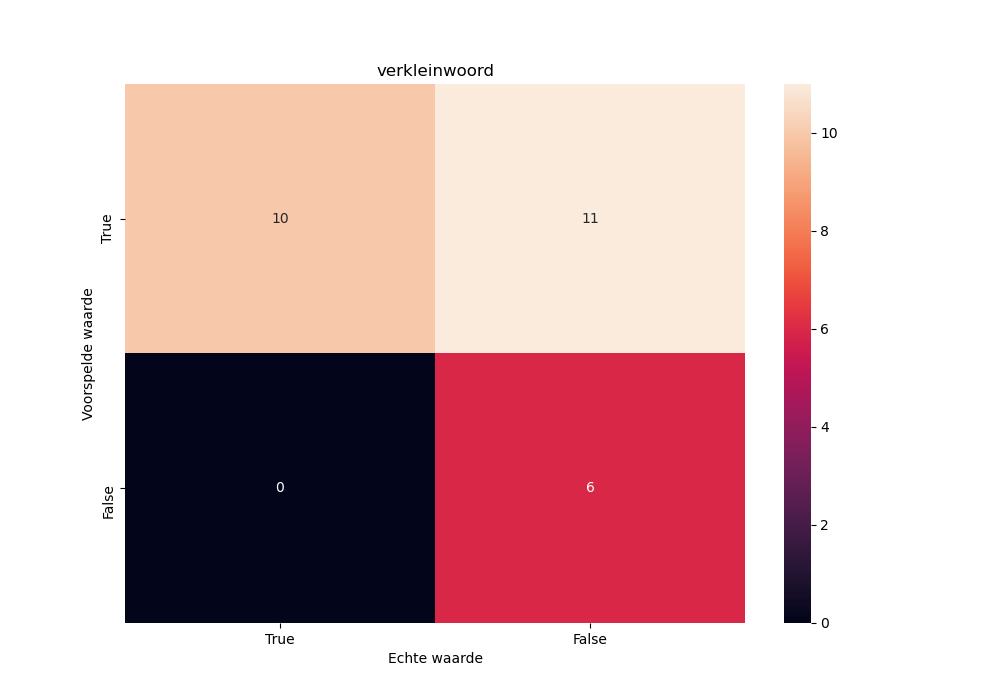
\includegraphics[width=1\textwidth]{./img/cfm_verkleinwoord}
    \caption{\label{fig:cfm_verkleinwoord} Resultaten \textit{confusion matrix} verkleinwoorden}
\end{figure}


\subsection{Toonhoogte}
De \textit{confusion matrix} van de testgevallen van de toonhoogte is te vinden in figuur~\ref{fig:cfm_pitch}.
\begin{figure}
    \centering
    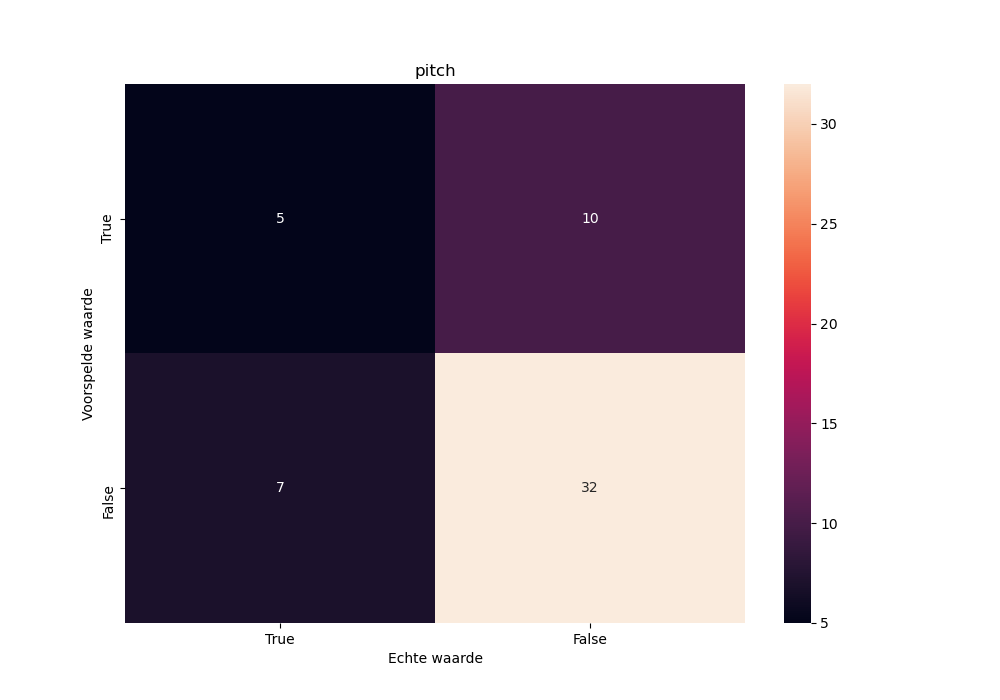
\includegraphics[width=1\textwidth]{./img/cfm_pitch}
    \caption{\label{fig:cfm_pitch} Resultaten \textit{confusion matrix} toonhoogte}
\end{figure}

\subsection{Stemvolume}

De \textit{confusion matrix} van de testgevallen van het stemvolume is te vinden in figuur~\ref{fig:cfm_pitch}.
\begin{figure}
    \centering
    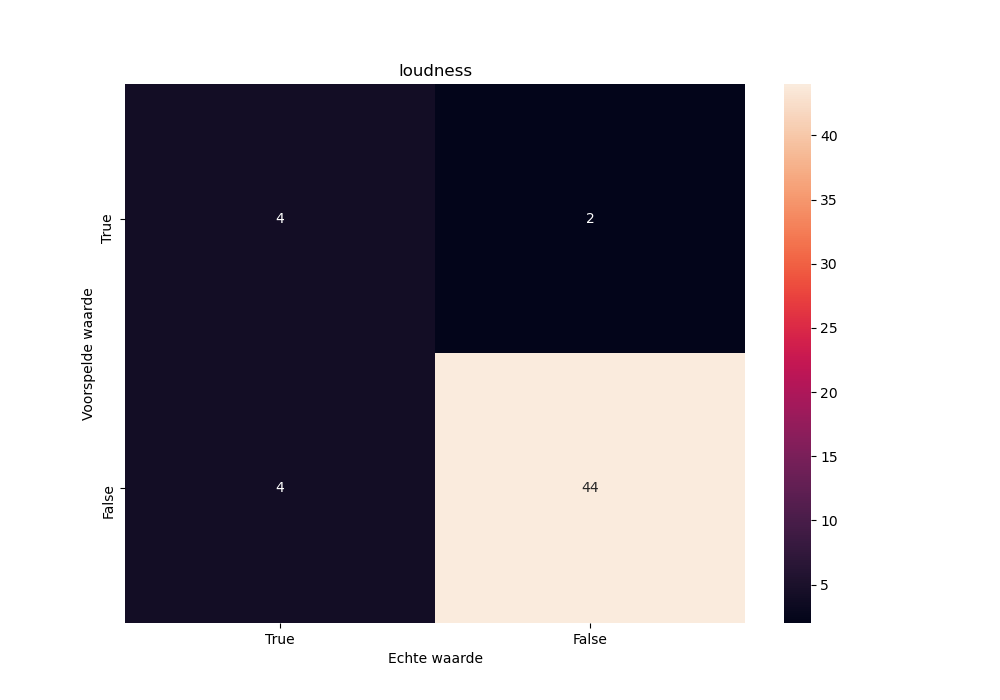
\includegraphics[width=1\textwidth]{./img/cfm_loudness}
    \caption{\label{fig:cfm_loudness} Resultaten \textit{confusion matrix} stemvolume}
\end{figure}


\section{Rollenspel}

\section{Zijn de requirements voldaan?}
%TODO: er is geen AI-model opgesteld
